\documentclass[t]{beamer}
\usetheme{Berkeley}
\setbeamertemplate{footline}[frame number]
\author{Peng-Wei CHEN}
\title{Zeros of Brownian motion}
\institute{MAP575 Foundations of probability and applications}
\AtBeginSection{\frame{\sectionpage}}

\begin{document}
\begin{frame}
    \titlepage
\end{frame}

\begin{frame}
    \tableofcontents
\end{frame}

\section{Fractal dimension}

\subsection{Definition}
\begin{frame}{Minkowski dimension}
    \begin{exampleblock}{Definition}
        Let $N(K, \varepsilon)$ be the minimal number of open balls of diameter $\varepsilon$ needed to cover a subset $K$ of a metric space.\\
        We define the upper Minkowski dimension as $$\overline{dim}_\mathcal{M}(K) = \limsup_{\varepsilon \to 0}\frac{\log N(K, \varepsilon)}{\log 1/\varepsilon}$$
        with $\liminf$ for the lower Minkowski dimension. Finally, we define $dim_\mathcal{M}(K)$ the Minkowski dimension if these two values agree.
        
    \end{exampleblock}
    \begin{itemize}
        \item Equal with two equivalent metric.
        \item{$N(k, \varepsilon) \sim C\varepsilon^{-dim_\mathcal{M}(K)}$}
        \item{Box counting dimension}
    \end{itemize}
\end{frame}

\begin{frame}{Minkowski dimension : examples}
    $$\dim_\mathcal{M}(K) = \lim_{\varepsilon \to 0}\frac{\log N(K, \varepsilon)}{\log 1/\varepsilon}$$
    \begin{exampleblock}{Exemples}
        $$
        \begin{array}{l|c c c c}
            & \mbox{Finite set} & $[0, 1]$ & \{0\}\cup \{1, \frac{1}{2}, \dots,\} \\
            \hline
            \mbox{Minkowski} & 0 & 1 & \frac{1}{2}\\
        \end{array}
        $$
    \end{exampleblock}
    %\pause
    %For $3^{-n} < \varepsilon \le 3^{-n+1}$, $2^{n-1} \le N(C_n, \varepsilon) < 2^{n}$.\\
    For $\frac{1}{n^2} < \varepsilon \le \frac{1}{(n+1)^2}$, $0, \frac{1}{n}, \frac{1}{n+1}\dots \in [0, \frac{1}{n}]$, $n \le N(K, \varepsilon) \le 2n + 1$.


\end{frame}

\begin{frame}{Hausdorff dimension}
    \begin{exampleblock}{Definition}
       We define the Hausdorff dimension of K as
       $$
       \dim(K) = \inf\left\{ \alpha: \underbrace{\inf \left\{ \sum_i |U_i|^\alpha : K \subset \bigcup_i U_i \right\}}_{\mathcal{H}^\alpha_\infty(K)} = 0 \right\}
       $$
    \end{exampleblock}
\end{frame}

\begin{frame}{Hausdorff dimension : examples}
    \begin{exampleblock}{Examples}
        $$
        \begin{array}{l|c c c c}
            & \mbox{Finite set} & $[0, 1]$ & \{0\}\cup \{1, \frac{1}{2}, \dots,\} \\
            \hline
            \mbox{Hausdorff} & 0 & 1 & 0\\
        \end{array}
        $$
    \end{exampleblock}
    \begin{itemize}
        \item $\varepsilon 2^{-n}$
        \item{For $\alpha > 1$, $\mathcal{H}^{\alpha}_{\infty}(K) = 0$}.
    \end{itemize}
\end{frame}

\begin{frame}{Mass Distribution Principle}
    \begin{block}{Lemma(Mass Distribution Principle)}
        If $\mu(B(x, r)) \le Cr^\alpha$ for a strictly positive Borel measure $\mu$ on E with a certain $C$ and $\alpha$, then
        $$
        \dim(E) \ge \alpha
        $$
    \end{block}
    $(U_i)_{i\in \mathbb{N}}$ so that $E \subset \bigcup_i U_i$, $(r_i)_{i\in \mathbb{N}}$ so that $|(U_i)| < r_i$.
    $$
    \mu(U_i) \le \mu\left( B(x_i, r_i) \right) \le C r_i^\alpha
    $$
    $$
    \sum_i |U_i|^\alpha \ge \sum_i \frac{\mu(U_i)}{C} \ge \frac{\mu(E)}{C} > 0
    $$
\end{frame}

\subsection{Comparison}
\begin{frame}{Comparison between the two dimensions}
    \begin{alertblock}{Definition}
    $$
    \lim_{\varepsilon \to 0} \frac{\log N(K, \varepsilon)}{\log 1/\varepsilon}\mbox{ and} \inf\left\{ \alpha:\mathcal{H}^\alpha_\infty (K) = 0 \right\}
    $$
    \end{alertblock}
    \begin{exampleblock}{Examples}
        $$
        \begin{array}{l| c c c c}
            & \mbox{Finite set} &[0, 1] & \{0\}\cup \{1, \frac{1}{2}, \dots,\} \\
            \hline
            \mbox{Minkowski} & 0 & 1 & \frac{1}{2}\\
            \mbox{Hausdorff} & 0 & 1 & 0\\
        \end{array}
        $$
    \end{exampleblock}
\end{frame}
\begin{frame}{Inequality}
    \begin{block}{Proposition}
        $\dim(K) \le \underline{\dim}_\mathcal{M}(K) \le \overline{\dim}_\mathcal{M}(K)$
    \end{block}
    $B_i = B(x_i, \frac{\varepsilon}{2})$, $N(K, \varepsilon)$ balls.\\
    For $\alpha > \underline{\dim}_\mathcal{M}$, $\sum_{i=1}^{N(K, \varepsilon)} |B_i|^\alpha = N(K, \varepsilon)\left( \frac{\varepsilon}{2}\right)^{\alpha} \le \frac{1}{2^\alpha} \varepsilon^{\alpha-\underline{\dim}_\mathcal{M}} \to 0$.
\end{frame}


\section{Zeros of the Brownian motion}
\begin{frame}{The fractal dimension of zeros of the Brownian motion}
    \begin{exampleblock}{Notation}
        We note $Z_B = \{t \in [0, +\infty) : B(t) = 0\}$ the set of zeros of the Brownian motion $B_t$.
    \end{exampleblock}
    \begin{block}{Theorem}
        With probability 1, dim$(Z_B) = \frac{1}{2}$.
    \end{block}
    $\frac{C}{\sqrt{\varepsilon}}$ balls.\\
    $\sum_{i} |U_i|^\alpha = 0$ for $\alpha > \frac{1}{2}$.

\end{frame}

\subsection{The lower bound for the fractal dimension}

\begin{frame}{Lower bound}
    \begin{block}{Lemma}
        With probability 1, 
        $$\dim\{t \in [0, 1] : Y(t) = 0\} \ge 1/2$$
        where $Y(t) = \max_{0\le s \le t} B_s - B_t$.
    \end{block}
    Let $M(t) = \max_{0\le s \le t} B_s$,\\$\mu([a, b]) = M(b) - M(a)$ define a measure with support strictly positive on $\{t \in [0, 1]: Y(t) = 0\}$.
    $$M(b) - M(a) \le \max_{0 \le h \le b-a} B_{a+h} - B_{a} \le C_\alpha (b-a)^\alpha$$
    \only<2>{
    \begin{block}{(Admitted), Hölder continuous}
        The Brownian motion is almost surely $\alpha$-Hölder continuous for $\alpha < 0.5$.
    \end{block}
    }
    \only<3->{
    \begin{alertblock}{Recall : Mass Distribution Principle}
        $\mu(B(x, r)) \le Cr^\alpha \to \dim(E) \ge \alpha$
    \end{alertblock}
    }
\end{frame}

\subsection{The upper bound for the fractal dimension}
\begin{frame}{The counter of a set}
    \only<1>{
    \begin{exampleblock}{The counter}
        We note
        $$N_m(A) = \sum_{k=1}^{2^m} 1_{A\cap [\frac{k-1}{2^m}, \frac{k}{2^m}] \neq \emptyset}$$
    \end{exampleblock}
    }
    \only<2->{
    \begin{block}{Lemma}
        Suppose $A$ is a closed random subset of $[0, 1]$ such that
        $$ \mathbb{E}[N_m(A)] \le c2^{m\alpha}$$
        for some $c, \alpha > 0$. Then $\overline{\dim}_\mathcal{M}(A) \le \alpha$.
    \end{block}
    $\mathbb{E}\left[ \sum_{m=1}^{\infty} \frac{N_m(A)}{2^{m(\alpha+\varepsilon)}} \right]$
    $ = \sum_{m=1}^{\infty} \frac{\mathbb{E} N_m(A)}{2^{m(\alpha+\varepsilon)}} < \infty$\\
    $\sum_{m=1}^{\infty} \frac{N_m(A)}{2^{m(\alpha+\varepsilon)}} < \infty$ a.s., 
    $\limsup_{m\to \infty} \frac{N_m(A)}{2^{m(\alpha+\varepsilon)}} = 0$
    $$
    \overline{\dim}_\mathcal{M}(A) = \limsup_{\varepsilon \to 0} \frac{\log N(A, \varepsilon)}{\log 1/\varepsilon} \le \limsup_{m \to \infty} \frac{\log(2^{m(\alpha+\varepsilon)})}{\log(2^m)} = \alpha + \varepsilon
    $$
    }
\end{frame}

\begin{frame}{The number of zeros in an interval}
    \begin{block}{Lemma}
        For any $a, \varepsilon > 0$ we have
        $$
        \mathbb{P}(\exists t \in (a, a+\varepsilon):B(t) = 0) \le C\sqrt{\frac{\varepsilon}{a+\varepsilon}}
        $$
    \end{block}
    Consider the event $A = \{ |B(a+\varepsilon)| \le \sqrt{\varepsilon} \}$.\\
    We have $\mathbb{P}(A) = \mathbb{P}\left( |B(1)| \le \sqrt{\frac{\varepsilon}{a+\varepsilon}} \right) \le 2\sqrt{\frac{\varepsilon}{a+\varepsilon}}$\\
    And 
    $$
    \begin{array}{r l}
        \mathbb{P}(A) & \ge \mathbb{P}\left( A \mbox{ and } 0 \in B_{[a, a+\varepsilon[} \right)\\
            & \ge \min_{a\le t \le a+\varepsilon} \mathbb{P}\left( A|B_t = 0 \right)\mathbb{P}\left( 0 \in B_{[a, a+\varepsilon[} \right)
    \end{array}
    $$
    Since $\mathbb{P}\left( |B_1| \le 1 \right) > 0$, we have
    $$
    \mathbb{P}\left( 0 \in B_{[a, a+\varepsilon[} \right) \le \frac{2}{c}\sqrt{\frac{\varepsilon}{a+\varepsilon}}
    $$

\end{frame}

\begin{frame}{The theorem}
    \begin{block}{Theorem}
        With probability 1, dim$(Z_B) = \frac{1}{2}$.
    \end{block}
    We have 
    $$
    \begin{array}{r l}
    \mathbb{E}\left[ N_m(Z_B) \right] &  = \sum_{k=1}^{2^m} \mathbb{P}\left( \exists t \in [\frac{k-1}{2^m}, \frac{k}{2^m}] : B(t) = 0 \right)\\
     & \le C\sum_{k=1}^{2^m} \frac{1}{\sqrt{k}}\\
     & \le \tilde{C} 2^{\frac{m}{2}}
    \end{array}
    $$
    \only<1>{
    \begin{block}{Lemma}
        For any $a, \varepsilon > 0$ we have
        $$
        \mathbb{P}(\exists t \in (\frac{k-1}{2^m}, \frac{k-1}{2^m}+\frac{1}{2^m}):B(t) = 0) \le C\sqrt{\frac{\frac{1}{2^m}}{\frac{k}{2^m}}}
        $$
    \end{block}
}
    \only<2>{
    \begin{block}{Lemma}
        Suppose $A$ is a closed random subset of $[0, 1]$ such that
        $$ \mathbb{E}[N_m(A)] \le c2^{m\alpha}$$
        for some $c, \alpha > 0$. Then $\overline{\dim}_\mathcal{M}(A) \le \alpha$.
    \end{block}
    Combine with the lower bound, we have thus $dim(Z_B) = \frac{1}{2}$ a.s.
}
\end{frame}

%\if 0
\section{Simulation results}

\begin{frame}{Some simulations for the Minkowski dimension}
    \begin{figure}
        \centering
        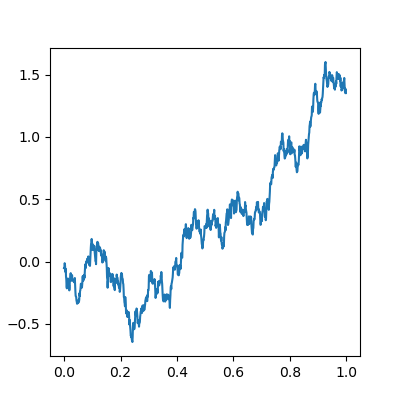
\includegraphics[scale=0.60]{brownian_motion.png}
        \caption{The brownian motion path}
        \label{fig:brownian_motion}
    \end{figure}
\end{frame}

\begin{frame}{Some simulations for the Minkowski dimension}
    \begin{figure}
        \centering
        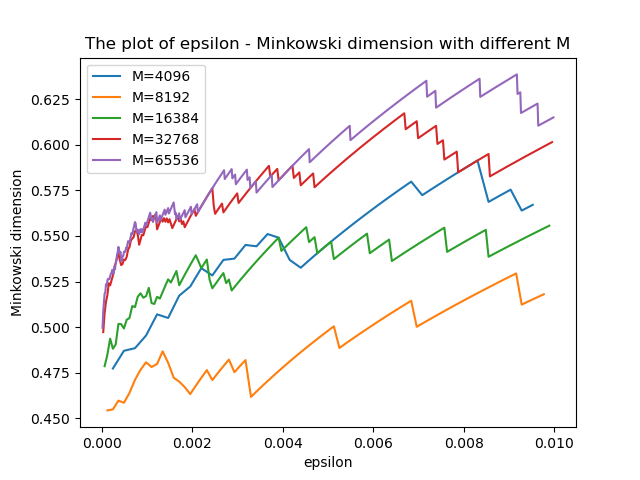
\includegraphics[scale=0.50]{differentM.png}
        \caption{Some examples with different length of step.}
        \label{fig:different_step}
    \end{figure}
\end{frame}

\begin{frame}{Some simulations for the Minkowski dimension}
    \begin{figure}
        \centering
        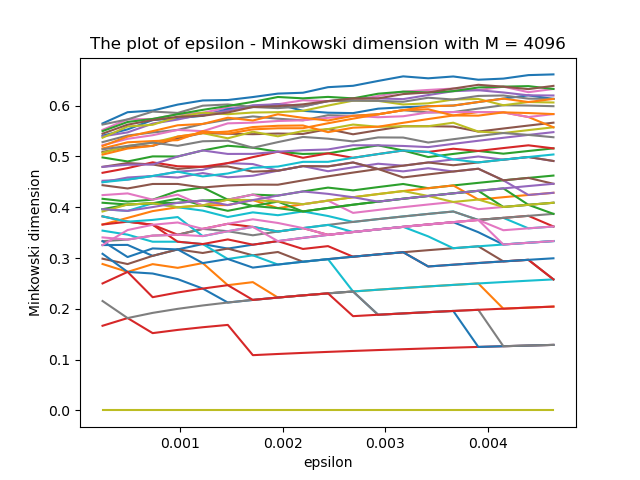
\includegraphics[scale=0.50]{sameM.png}
        \caption{Some examples with same length of step.}
        \label{fig:same_step}
    \end{figure}
\end{frame}

\begin{frame}{Some simulations for the Minkowski dimension}
    \begin{figure}
        \centering
        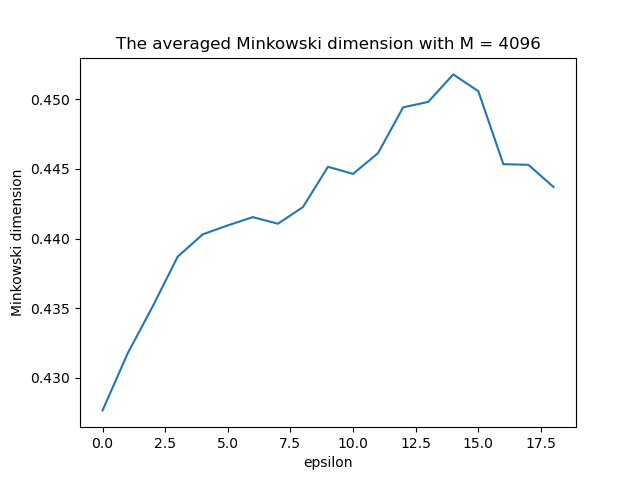
\includegraphics[scale=0.50]{mean.png}
        \caption{The distribution of the average Minkowski dimension.}
        \label{fig:average}
    \end{figure}
\end{frame}

\begin{frame}{Some simulations for the Minkowski dimension}
    \begin{figure}
        \centering
        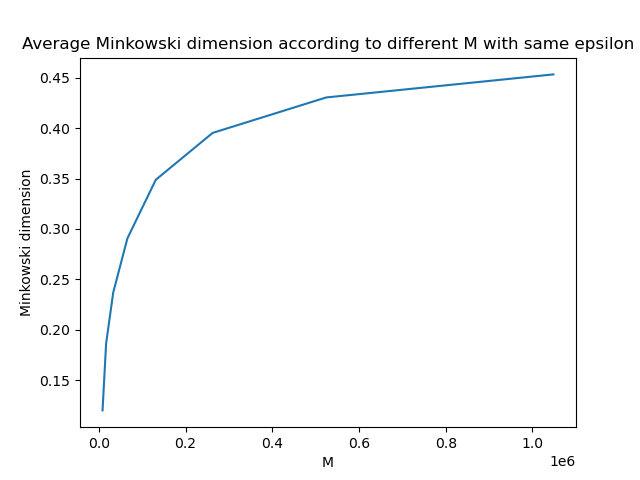
\includegraphics[scale=0.50]{differentM_2.png}
        \caption{Average Minkowski dimension according to different M with same epsilon}
        \label{fig:same_eps}
    \end{figure}
\end{frame}
%\fi

\begin{frame}{Thanks!}
    
\end{frame}

\end{document}
